% Video slides (13). Build in a folder that also holds the course slide file saved as course.pdf
% (a copy of week4coursework-combined.pdf):
%   pdflatex slides.tex && pdflatex slides.tex
% Slides 2 and 3 are pages 16 and 6 of the course slides, credited on the slide.
% Keep this file anonymous: no names, UUNs, group IDs or repository links.
\documentclass[aspectratio=169,12pt]{beamer}
\usepackage{pgfplots}
\usepackage{booktabs}
\pgfplotsset{compat=1.16}
\usetheme{default}
\usecolortheme{default}
\setbeamertemplate{navigation symbols}{}
\setbeamerfont{frametitle}{size=\LARGE,series=\bfseries}
\setbeamerfont{normal text}{size=\large}
\setbeamertemplate{footline}[frame number]
\pdfinfo{/Title () /Author ()}
% A full course slide with a small credit in the bottom-right corner.
\newcommand{\course}[2]{\begin{frame}[plain]
\begin{tikzpicture}[remember picture,overlay]
\node at (current page.center) {\includegraphics[page=#1,width=\paperwidth,height=\paperheight,keepaspectratio]{course.pdf}};
\node[anchor=south east,fill=white,fill opacity=0.85,text opacity=1,font=\scriptsize,inner sep=2pt] at (current page.south east) {Source: course slides (Week 4), ``#2''};
\end{tikzpicture}
\end{frame}}

\begin{document}

% ---- 1 Title
\begin{frame}[plain]
\vfill\centering
{\Huge\bfseries Where the time\\[3mm] and the evidence go\par}\vspace{8mm}
{\Large CUDA kernels and retrieval depth\\in a spoken-question answering system}\\[12mm]
{\large Machine Learning Systems coursework}
\vfill
\end{frame}

% ---- 2 Course slide: the pipeline
\course{16}{The common pipeline}

% ---- 3 Course slide: where kernels run
\course{6}{Inside one layer}

% ---- 4 What we built
\begin{frame}{What we built}
\begin{itemize}
\item[] \textbf{Speech side: four GPU kernels (CUDA)}
\begin{itemize}
\item \textbf{RoPE}: marks each token's position
\item \textbf{Reductions}: sums and maximums, used by RMSNorm and softmax
\item \textbf{GEMM}: the matrix multiply (86\% of the GPU time)
\item \textbf{Attention}: lets each token look at the others
\end{itemize}
\vspace{3mm}
\item[] \textbf{Answering side: our own experiment scripts}
\begin{itemize}
\item cache the speech transcripts once, so every test sees the same text
\item measure retrieval depth $k$: quality and cost
\item one idea of our own: \textbf{adaptive $k$}
\end{itemize}
\end{itemize}
\end{frame}

% ---- 5 ASR results
\begin{frame}{Speech: correct, but slower than PyTorch}
\textbf{Same GPU, same job (RTX 2080 Ti), 3.5\,s test recording}\\[3mm]
\begin{tabular}{lrr}
\toprule
 & ms per transcription & transcript\\
\midrule
PyTorch (cuBLAS inside) & 1096 & exact\\
Our four kernels & 2699 & exact\\
\bottomrule
\end{tabular}\\[2mm]
\textbf{Ours is 2.45$\times$ slower.}\\[5mm]
\textbf{Why?} Where the GPU time goes with our kernels:\\[1mm]
\begin{tabular}{lr}
matrix multiply (GEMM) & 86\%\\
attention & 13\%\\
everything else & under 1\%\\
\end{tabular}
\end{frame}

% ---- 6 GEMM
\begin{frame}{The matrix multiply: naive vs ours vs cuBLAS}
Speed in GFLOP/s (higher is better), big encoder layer:\\[3mm]
\begin{tabular}{lrr}
\toprule
naive kernel & 233 & \\
\textbf{our tiled kernel} & \textbf{2107} & 9$\times$ faster than naive\\
cuBLAS (NVIDIA library) & 13363 & 6$\times$ faster than ours\\
\bottomrule
\end{tabular}\\[5mm]
\begin{itemize}
\item Tiles in fast shared memory: each value is loaded once per tile and reused 32 times.
\item cuBLAS also keeps several results per thread in registers: that is the gap.
\end{itemize}
\end{frame}

% ---- 7 Our question
\begin{frame}{Our question about answering}
\textbf{How many retrieved records ($k$) should the answer model get? What does extra depth cost?}\\[4mm]
\begin{itemize}
\item Same cached transcripts for every test: only $k$ changes.
\item Retrieval quality: 350 practice and 125 dev questions.
\item Answer quality (an AI judge, score 0 to 1): 28 practice + 27 held-out dev questions, the same ones at every $k$.
\item Cost: prompt size, time to write the answer.
\end{itemize}
\end{frame}

% ---- 8 Recall vs k
\begin{frame}{More records find more of the right ones}
\begin{center}
\begin{tikzpicture}
\begin{axis}[width=0.6\textwidth,height=0.62\textheight,xmode=log,log basis x=10,
 xtick={1,5,20,100},xticklabels={1,5,20,100},xlabel={records retrieved ($k$)},
 ylabel={share (0 to 1)},ymin=0,ymax=1,legend pos=outer north east,legend cell align=left,grid=major,
 every axis plot/.append style={thick}]
\addplot[blue,mark=*] coordinates {(1,0.229)(5,0.421)(10,0.480)(20,0.579)(50,0.684)(100,0.770)};
\addlegendentry{Recall@$k$}
\addplot[red,mark=square*] coordinates {(1,0.411)(5,0.591)(10,0.651)(20,0.737)(50,0.820)(100,0.880)};
\addlegendentry{at least one right record}
\end{axis}
\end{tikzpicture}
\end{center}
\centering Practice split, 350 questions. Searching all 24{,}000 records takes about 0.5\,ms whatever $k$ is.\\
But 12\% of questions never reach a right record, even at $k=100$.
\end{frame}

% ---- 9 Judge score vs k
\begin{frame}{But better answers? No visible difference}
\begin{columns}
\column{0.58\textwidth}
\begin{tikzpicture}
\begin{axis}[width=\textwidth,height=0.6\textheight,symbolic x coords={1,5,20},xtick=data,
 xlabel={records retrieved ($k$)},ylabel={judge score (0 to 1)},ymin=0,ymax=0.6,grid=major,
 enlarge x limits=0.3]
\addplot[only marks,mark=*,mark size=3pt,blue,error bars/.cd,y dir=both,y explicit]
 coordinates {(1,0.267) +- (0,0.088) (5,0.294) +- (0,0.085) (20,0.273) +- (0,0.093)};
\end{axis}
\end{tikzpicture}
\column{0.4\textwidth}
\small 55 questions, bars = 95\% range\\[2mm]
\begin{tabular}{lrr}
\toprule
$k$ & prompt tokens & seconds\\
\midrule
1 & 310 & 1.9\\
5 & 1137 & 4.7\\
20 & 4544 & 6.4\\
\bottomrule
\end{tabular}\\[2mm]
Prompt grows $15\times$.\\ Score differences: at most 0.03.\\ We cannot see a difference smaller than about 0.09.
\end{columns}
\end{frame}

% ---- 10 Why: coverage vs dilution
\begin{frame}{Why? Two effects cancel}
Judge score, 28 practice questions, grouped by where the first right record is ranked:\\[3mm]
\begin{tabular}{lrccc}
\toprule
first right record at & questions & $k=1$ & $k=5$ & $k=20$\\
\midrule
rank 1 & 11 & \textbf{0.45} & 0.39 & 0.39\\
ranks 2--5 & 8 & 0.21 & 0.25 & \textbf{0.34}\\
ranks 6--20 & 4 & 0.10 & 0.29 & 0.29\\
not in top 20 & 5 & 0 & 0 & 0\\
\bottomrule
\end{tabular}\\[4mm]
\begin{itemize}
\item Right record already first: extra records only distract.
\item Right record lower: extra records help.
\item Not found at all: no $k$ helps.
\end{itemize}
{\small Small groups, made after seeing the data. On held-out dev, rank-1 questions again lose with more records.}
\end{frame}

% ---- 11 Adaptive k
\begin{frame}{Our own idea: adaptive $k$. It does not help.}
Rule: if the top two scores are far apart, use $k=1$; otherwise $k=20$. Tuned on practice, tested on held-out dev.\\[3mm]
\begin{tabular}{lrr}
\toprule
 (dev, 27 questions) & judge score & prompt tokens\\
\midrule
always $k=5$ & \textbf{0.321} & 1022\\
always $k=20$ & 0.253 & 4351\\
\textbf{adaptive} & 0.272 & 3367\\
perfect gate (oracle) & 0.306 & 2419\\
\bottomrule
\end{tabular}\\[4mm]
\begin{itemize}
\item The gate is weak: about a third of its ``confident'' questions have the wrong top record.
\item Even a perfect gate gains little: a quarter of questions have no right record in the top 20.
\end{itemize}
\end{frame}

% ---- 12 Question 1
\begin{frame}{Question 1: our main design choice}
\textbf{We tuned only what the profile said matters.}
\begin{itemize}
\item Profile (handout settings): matrix multiply 84\%, attention 16\%, the rest under 1\%.
\item So we tuned only those two: tile 32 (not 16), 16 queries per attention block (not 4).
\item Result: 17\% faster (3294 $\to$ 2728\,ms), transcript still exact.
\item Cost we accept: one tile size does not fit every shape (the one-row output layer is slower).
\end{itemize}
\end{frame}

% ---- 13 Question 2
\begin{frame}{Question 2: how we checked our work}
\begin{itemize}
\item Course tests: every kernel against a CPU / cuBLAS answer, including edge cases.
\item Sanitizer: no memory errors, no race conditions.
\item Full model: the transcript must be exactly right.
\item Repeated runs on different nodes: our time varies under 1\%.
\end{itemize}
\textbf{Example 1:} fast-math looked like free speed, but a RoPE test failed: rejected.\\
\textbf{Example 2:} after 15 questions $k=20$ looked better; with 13 more it vanished: claim withdrawn.
\end{frame}

\end{document}
